\documentclass{article}
\usepackage[dvipsnames]{xcolor}
\usepackage[paperwidth=20cm, paperheight=6cm, margin = 0cm, top=0.5cm]{geometry}
\usepackage{amsmath}


\usepackage{pgf}
\usepackage{tikz}
\usetikzlibrary{positioning, calc}
\usetikzlibrary{arrows,automata}

\tikzstyle{source}  = 
[
	draw,circle,fill=black,thick,inner sep=0mm,minimum size=2mm
]

\tikzstyle{box}  =
[
	draw,rectangle,thick,inner sep=2mm,
	minimum width=8mm, minimum height=8mm
]

\tikzstyle{redbox} = 
[
	draw,rectangle,thick,inner sep=2mm,
	minimum width=8mm, minimum height=8mm,
	fill=red, opacity=0.3, text opacity=1, draw opacity=1
]

\tikzstyle{dredbox} = 
[
	draw,rectangle,thick,inner sep=2mm,
	minimum width=8mm, minimum height=8mm,
	fill=red, opacity=0.5, text opacity=1, draw opacity=1
]


\tikzstyle{bluebox} = 
[
	draw,rectangle,thick,inner sep=2mm,
	minimum width=8mm, minimum height=8mm,
	fill=blue, opacity=0.3, text opacity=1, draw opacity=1
]

\tikzstyle{greenbox} = 
[
	draw,rectangle,thick,inner sep=2mm,
	minimum width=8mm, minimum height=8mm,
	fill=green, opacity=0.3, text opacity=1, draw opacity=1
]

\tikzstyle{lgreenbox} = 
[
	draw,rectangle,thick,inner sep=2mm,
	minimum width=8mm, minimum height=8mm,
	fill=SpringGreen
]

\tikzstyle{dgreenbox} = 
[
	draw,rectangle,thick,inner sep=2mm,
	minimum width=8mm, minimum height=8mm,
	fill=ForestGreen, opacity=0.5, text opacity=1, draw opacity=1
]


\tikzstyle{bluestate}  = 
[
	state, draw=blue, line width=2pt,
	fill=LimeGreen
]

\tikzstyle{redstate}  = 
[
	state, draw=red, line width=2pt,
	fill=LimeGreen
]

\tikzstyle{violetstate}  = 
[
	state, draw=Violet, line width=2pt,
	fill=LimeGreen
]



\renewcommand{\vec}[1]{\boldsymbol{#1}}

\begin{document}
\begin{center}
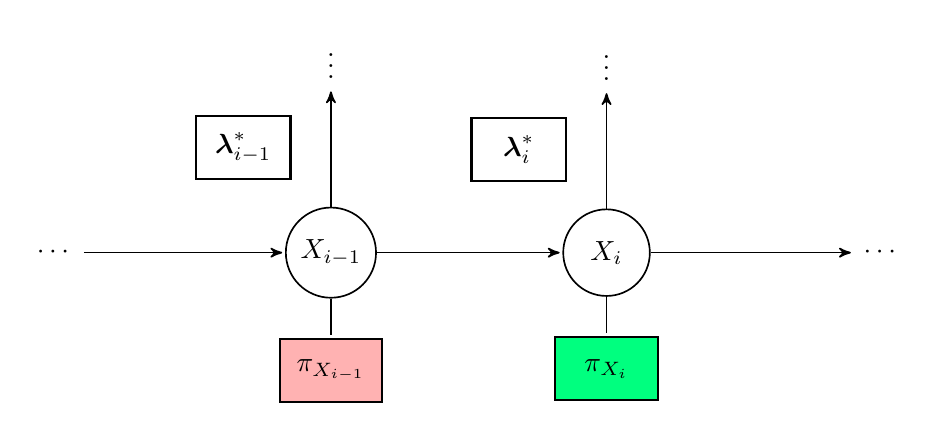
\begin{tikzpicture}[->,>=stealth',shorten >=1pt,auto,node distance=3.5cm,semithick]
                    
\node (X0)               {$\cdots$}; 
\node[state, minimum size=1.1cm] (X1) [right of=X0] {$X_{i-1}$}; 
\node[state, minimum size=1.1cm] (X2) [right of=X1] {$X_{i}$};                   
\node (X3) [right of=X2] {$\cdots$};                   

\node (Y1) [above=1.5cm of X1] {$\vdots$}; 
\node (Y2) [above=1.5cm of X2] {$\vdots$}; 

\node[redbox, minimum width=1.3cm] (P1) [below=0.5cm of X1] {$\pi_{X_{i-1}}$}; 
\node[lgreenbox, minimum width=1.3cm] (P2) [below=0.5cm of X2] {$\pi_{X_{i}}$}; 
		
\path
    (X0) edge (X1)  
	(X1) edge (X2)
	(X2) edge (X3);
	
\path	
	(X1) edge node[box, xshift=-0.5cm, minimum width=1.2cm] {$\vec{\lambda}_{i-1}^*$} (Y1)
	(X2) edge node[box, xshift=-0.5cm, minimum width=1.2cm] {$\vec{\lambda}_{i}^*$}(Y2);

\path
	(X1) edge[-] (P1)
	(X2) edge[-] (P2);


\end{tikzpicture}
\end{center}

\end{document}
